%
% Refrence http://en.wikibooks.org/wiki/LaTeX
%

\documentclass[10pt]{article}

% ======
% Header
% ======

% use droid sans
\usepackage{droidsans}    
\renewcommand\familydefault{\sfdefault}   % set default font to sans-serif


% enable \href
\usepackage[colorlinks=true,
            linkcolor=blue,
            urlcolor=blue,
            allbordercolors={0 0 0},
            pdfborderstyle={/S/U/W 1}]{hyperref}

% enable \includegraphics for embedding jpgs
\usepackage{graphicx}  

% ==================
% Document Meta Data
% ==================

\title{Webtech Report}
\author{Imna Malik n James Sewart}
\date{29-5-16}

% ====
% Body
% ====

\begin{document}

    \maketitle

    \tableofcontents


    \begin{abstract}
        The \href{https://smple.uk}{Smple} (short for sample) web application is a visual geospatial music discovery service. Users can discover new artists playing in their area and sample their music using data gathered from the Internet.
    \end{abstract}

    \section{Client}
        \subsection{Style}
            The web app is designed to be used on modern browsers and is tested on the latest Safari for OS X, Firefox, Chrome, and Safari for iOS. We do not support old IE.
            \subsubsection{General Layout}
                \begin{figure}[!ht]
                  \centering
                    \reflectbox{
                      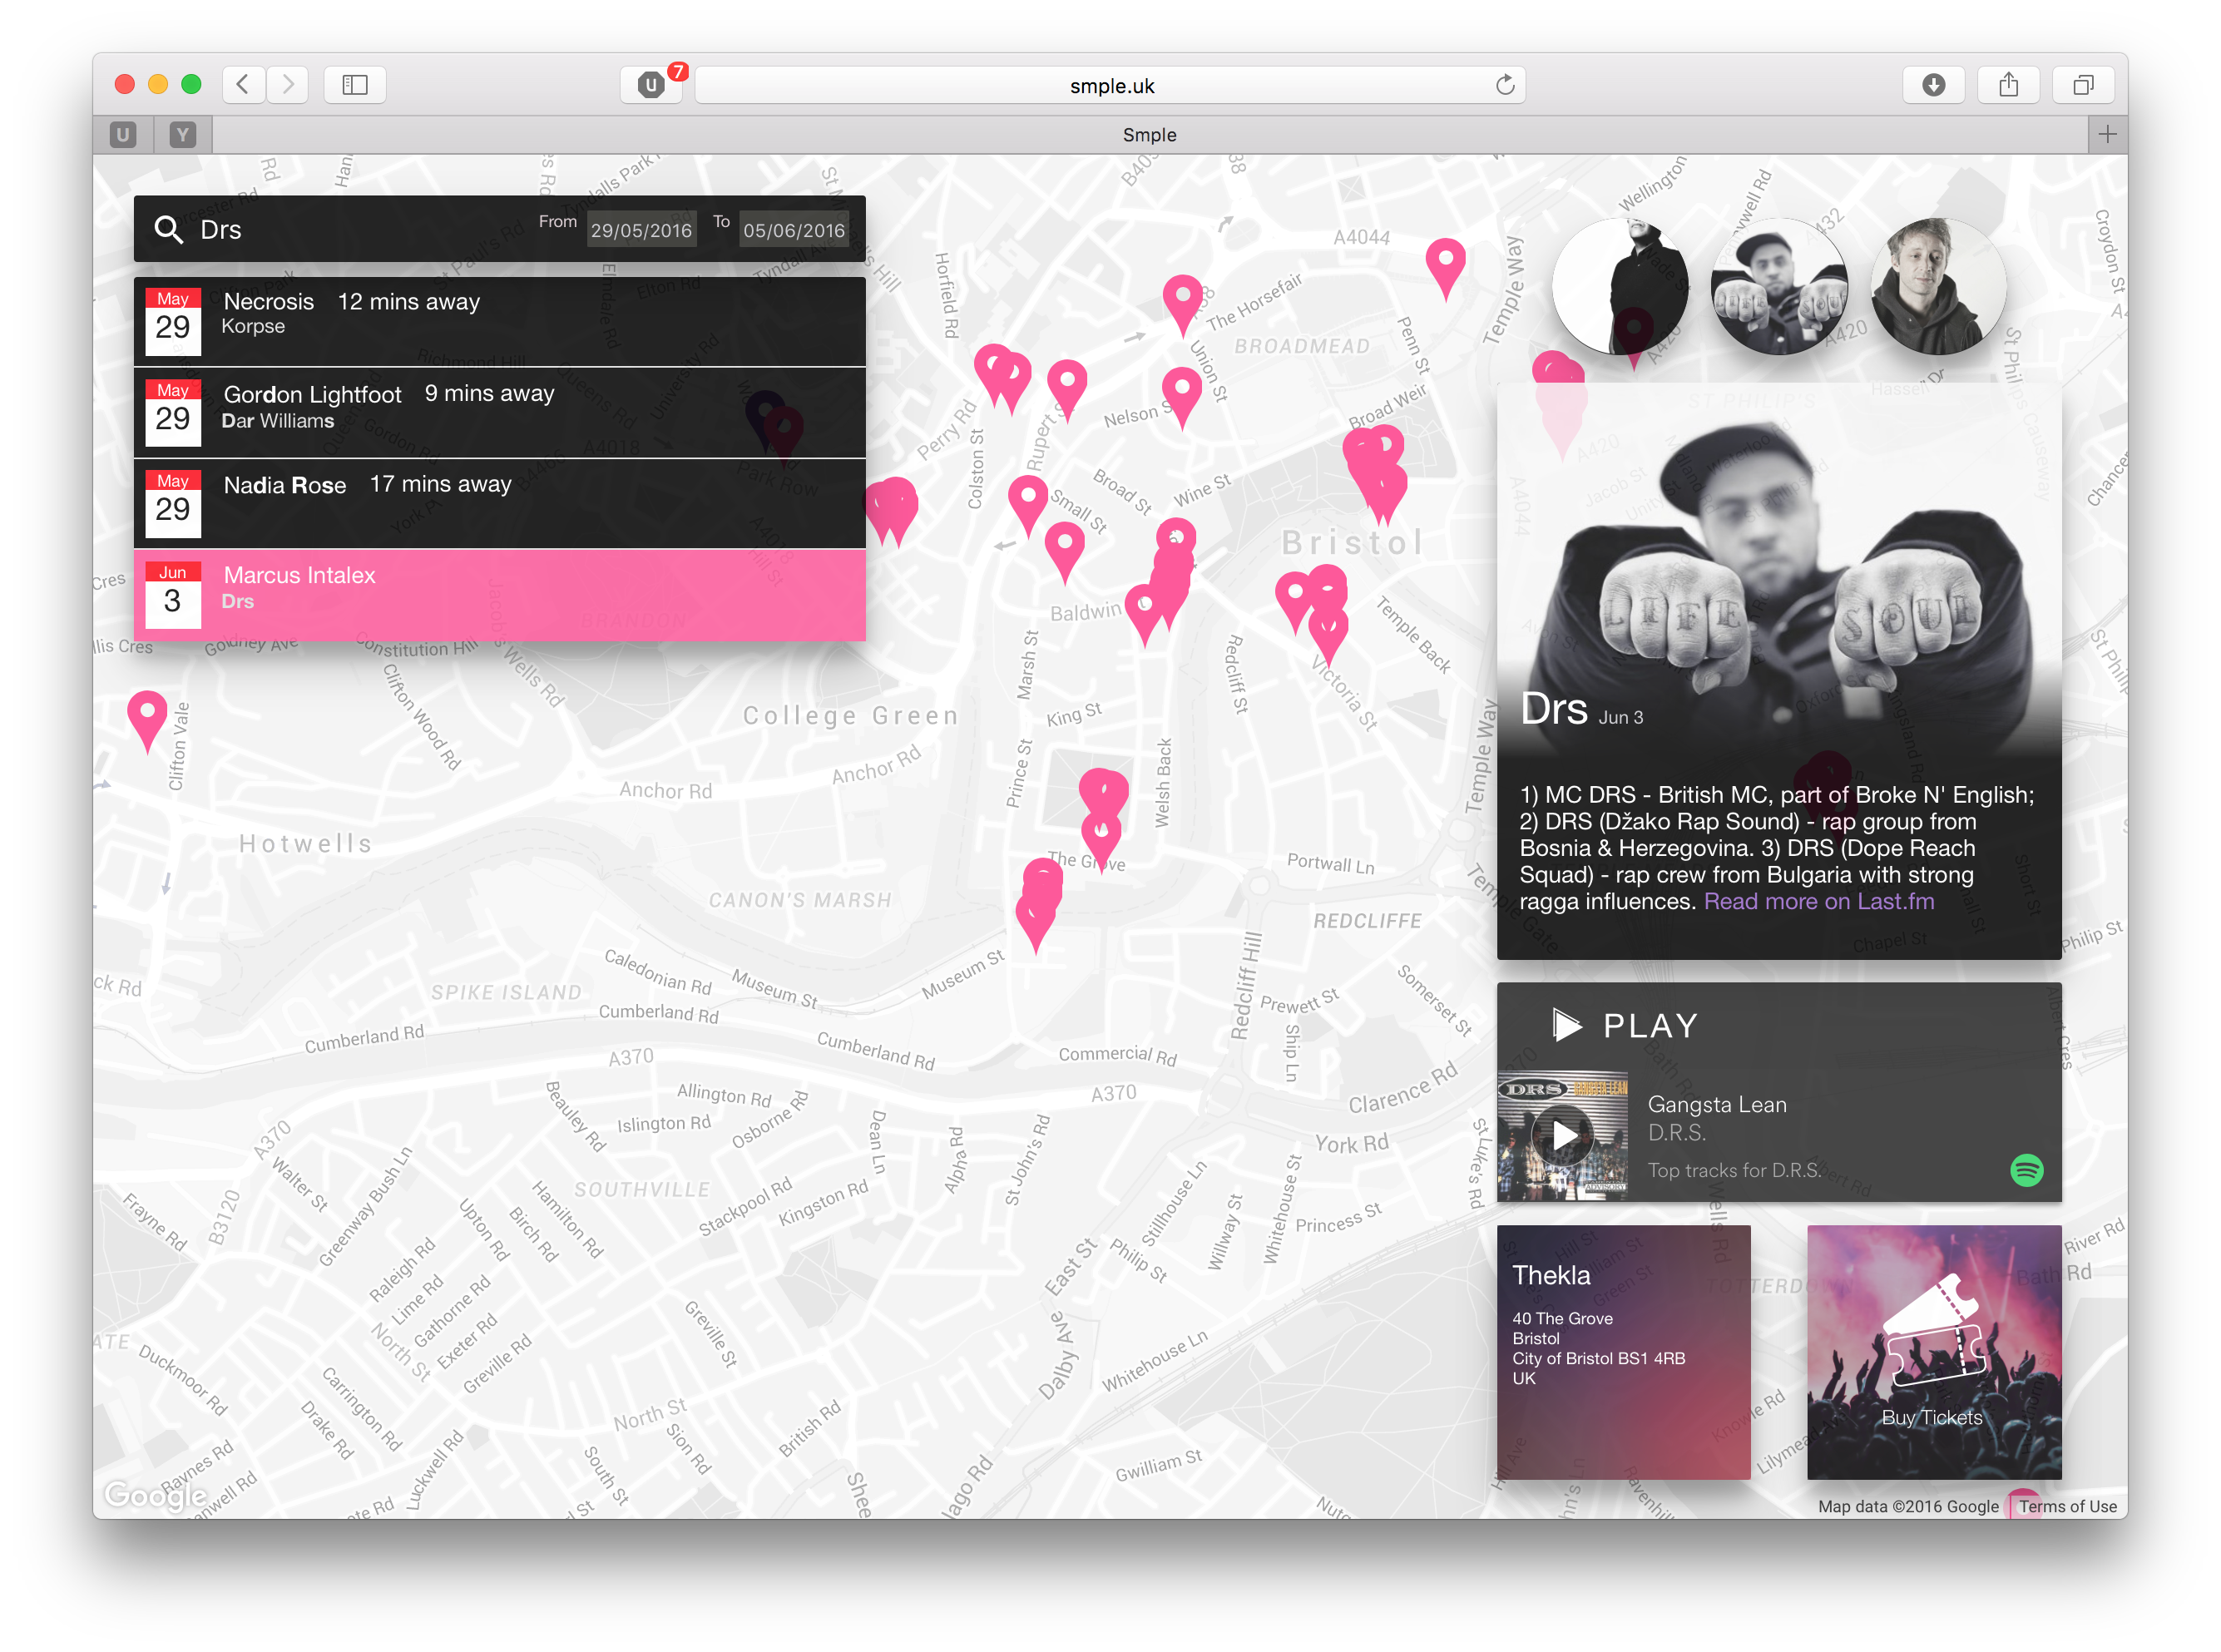
\includegraphics[height=60mm]{example1.png}}
                  \caption{Basic layout description.}
                \end{figure}

                The Smple web application consists of a single page filled with a map from the Google Maps API. There are two panels: the search on the left, and the information (info) on the right. 

                The search panel consists of an input to type a query and two date pickers to choose the date range for events to be displayed. When a search query is made results are shown underneath with their event date, band names, and the time to walk there.

                When an event is selected by clicking a marker or search result, the info panel slides into view from the right. At the top, the artist thumbnails are displayed. They are dynamically created depending on how many artists are playing in the selected event. Below, is the artist name, image, and biography for the selected artist. If the play button underneath is clicked, an embedded Spotify player is shown. Lastly is the events venue address and the link to the ticket-sale website which are contained in their individual panels.

                There are two markers present on the map: pink and purple. The pink markers represent events and the purple is used to indicate the current user location which is determined by the browser.

               If the map is moved or zoomed, the info panel will slide out of view. Additionally, when the info panel's content overflows the bottom of the page, it becomes scrollable.


            \subsubsection{Base Classes}
                The design of our layout is inspired by Material Design with it's iconic card styled boxes. Each panel is given a shadowbox class which gives the element a border radius, shadow, slight transparency, and a dark background colour. The search panel and the panels within the info panel are styled with this class.

            \subsubsection{Resizing}
                CSS media queries are used to change large scale layouts based on the screen width. There are three of these: mobile-size, large, and extra large. These changes involve setting the widths of the main panels such that they look good on the screen size. For the mobile screen this means the panels are full width and stack on top of each other. For the large size the info bar takes up a third of the screen, and the search 40\% of the screen.

                For a more dynamic resize control we subscribe to the onresize event of the window and scale the whole document's font size based on the screen width in JavaScript. Most elements are defined using ems and so they all scale accordingly.
                \begin{figure}[!ht]
                  \centering
                    \reflectbox{
                      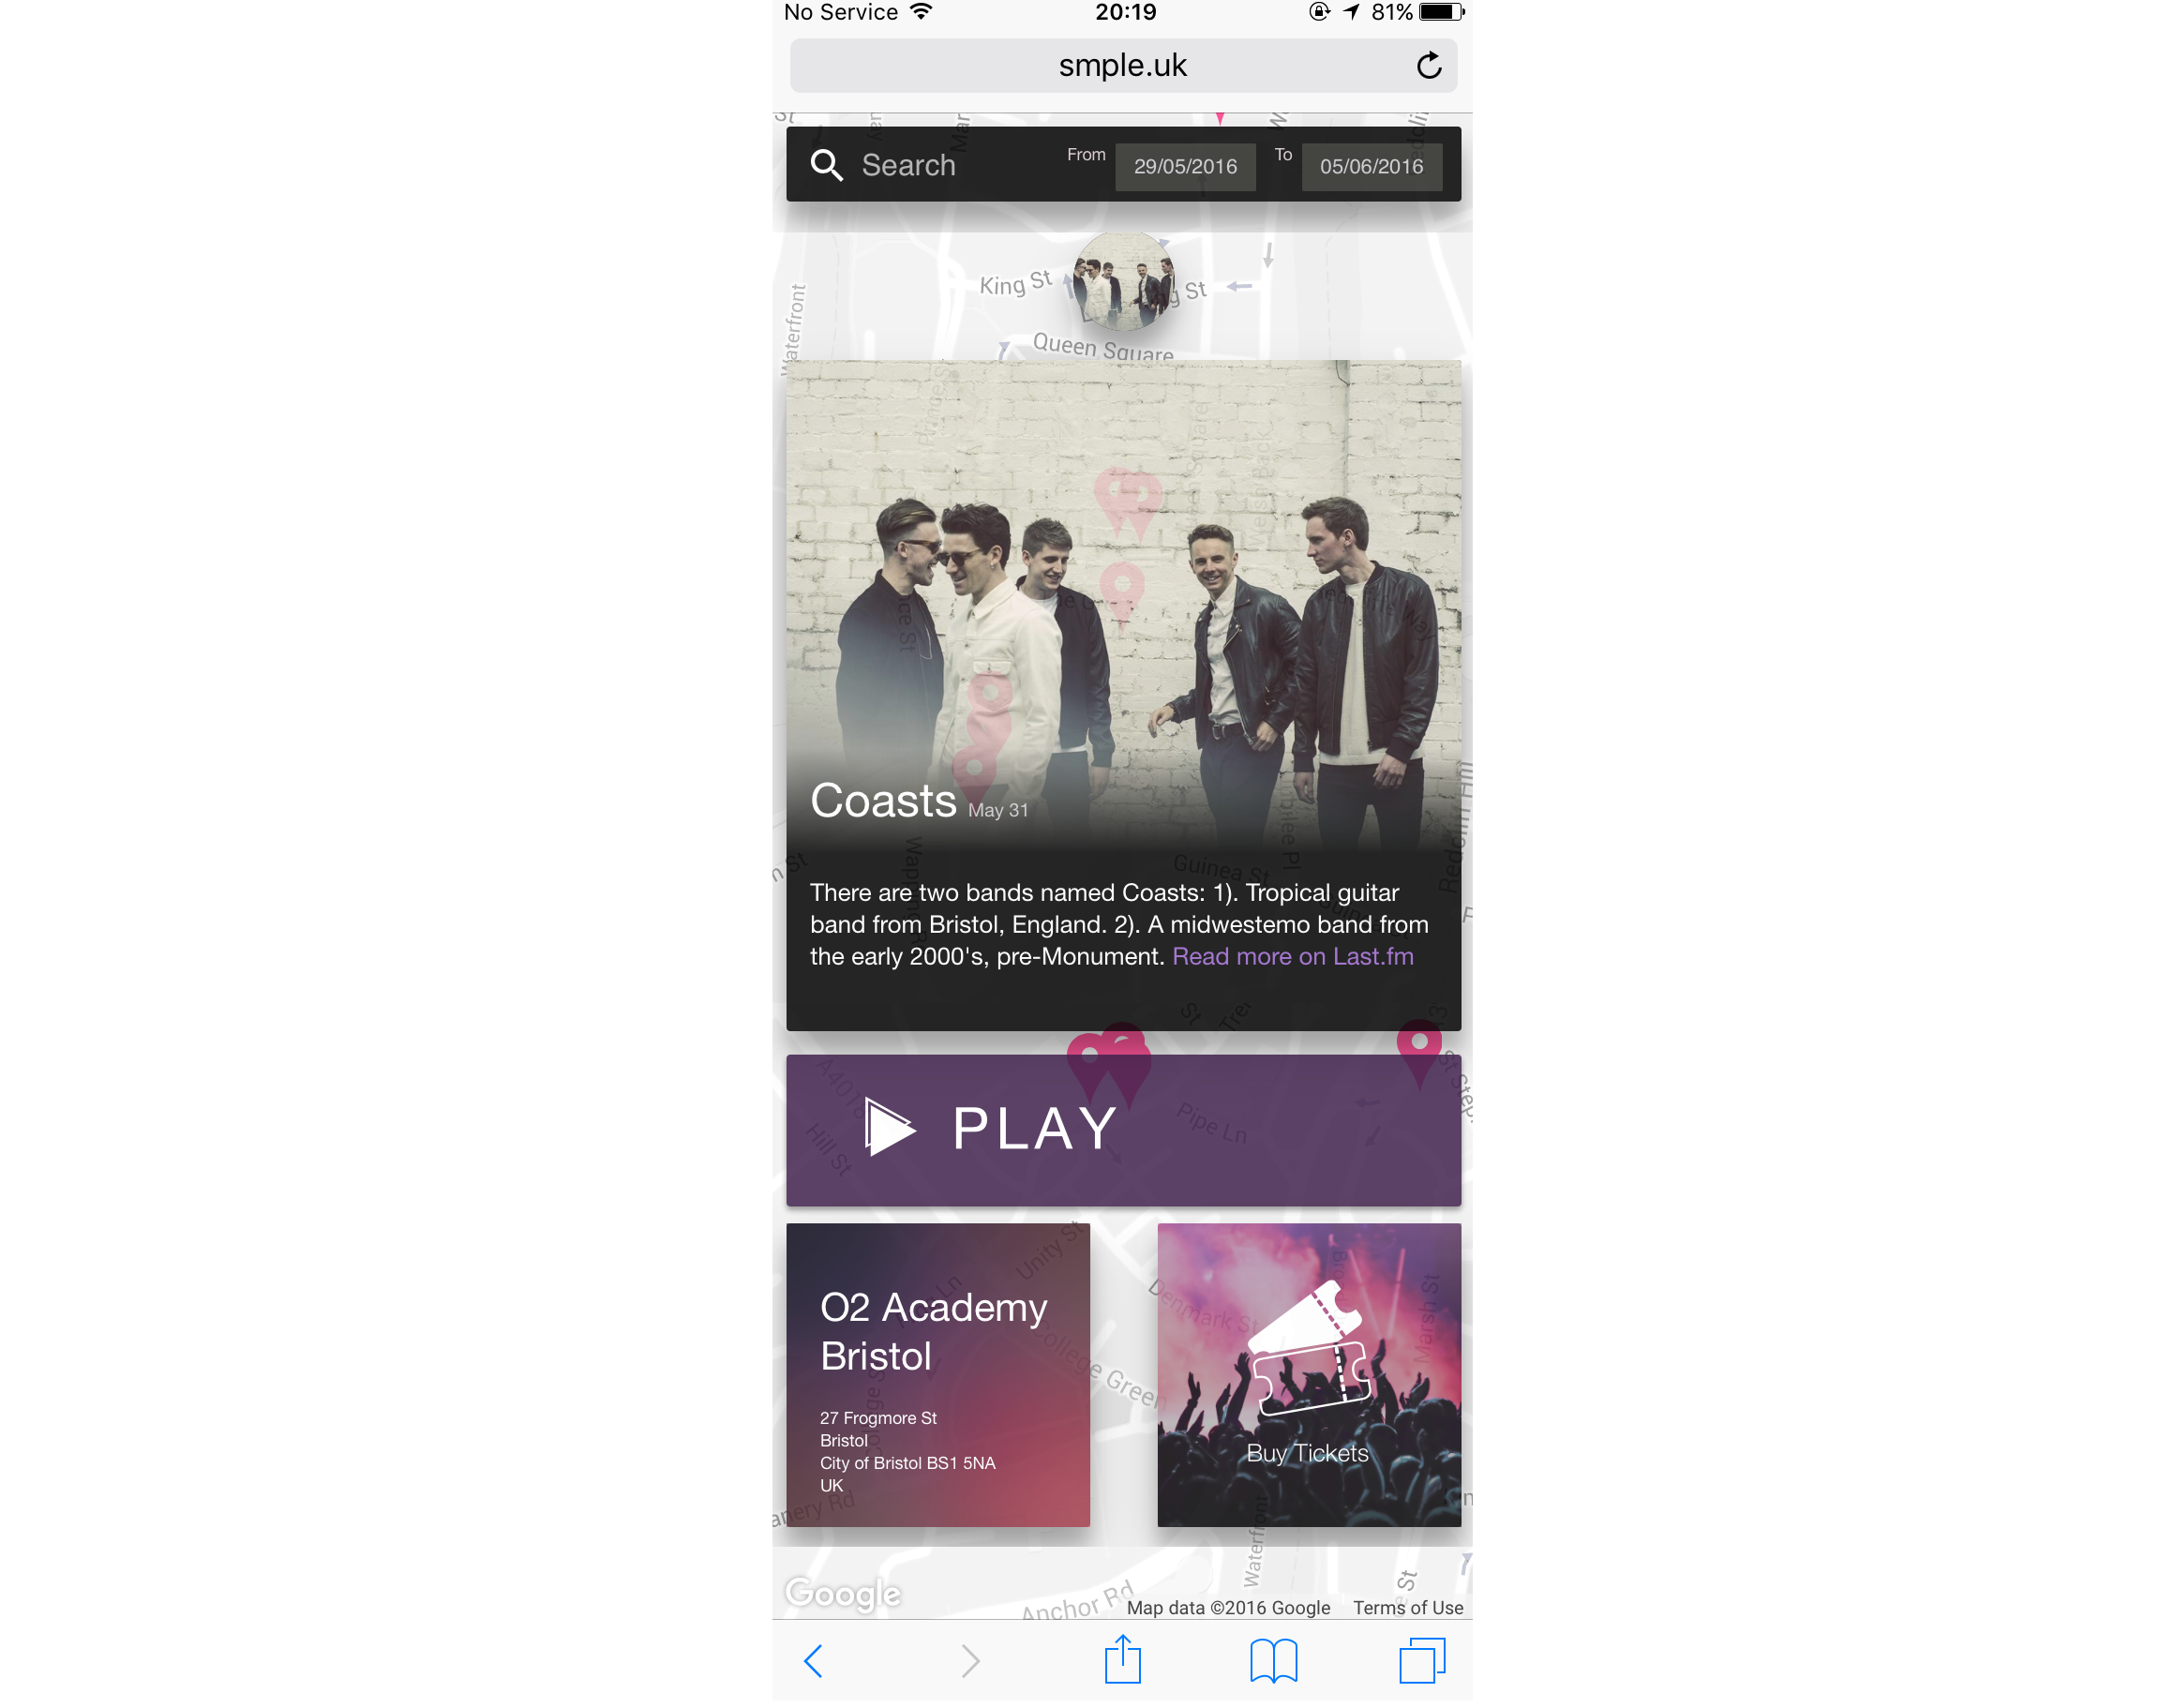
\includegraphics[height=60mm]{example3.png}}
                  \caption{Example layout when rendered using a mobile browser.}
                \end{figure}

            \subsubsection{Info Panel}
                The info panel involves many different styling and scripting elements. Animations in the panel are done using the CSS transition property and setting the margin-right to 0 from -33\%. By default, moving this panel to the right would bring up a scrolling bar. However this is prevented by setting the overflow property to hidden.

                Initially, the animation's performance was poor in early development due interaction with the map styling. This caused a browser reflow to happen for every frame of the animation. Our research determined that we needed to avoid as many reflows as possible when animating for best performance. Changing the map to be position:absolute significantly improved performance as only repaints were necessary.

                In order to produce the desired scrolling effect, we set the overflow-y property to scroll. This allows the contents to scroll within its div. To ensure that the content does not increase the page size, the height is set to 100\% of the screen height.

                Artist thumbnails are contained within an element with text-align set to center. Each image is an inline-block to allow overflow and centering independent of the number of thumbnails. Since the images could be of any aspect ratio, we use the object-fit CSS property which is set as cover, and the left and top property which is set as 50\% to keep the thumbnail container filled and the image centered inside. The container is given a border radius of 50\% to create a circular thumbnail, and the overflow is set to hidden to crop the image inside. Furthermore, the thumbnail is animated to zoom on hover using a CSS selector that transforms the scale of the thumbnail container.

                Missing artists have a silhouette avatar picture as their thumbnail. This was created by finding a silhouette SVG found online and overlaying it on-top of a gradient PNG image which was imported into Inkscape with the image rendering mode set to smooth to ensure the best quality conversion. 

                The box underneath contains an element for the artist title, along with a paragraph tag for the biography. The title is displayed over the artist image and has a gradient behind it to make sure the text is visible. Additionally, the title is pinned to the bottom of the image. The image width is set to the parent's width so that only the height changes depending on the aspect ratio. This height pushes down the biography accordingly. For aesthetic purposes, there is a padding set on the biography.

                Beneath the artist information box is a purple SVG button. When clicked, it triggers a set of animations. The two triangles will turn 120 degrees clockwise with slightly different durations using SMIL animations. Also, the size of the box increases to reveal an iframe with a Spotify embedded player inside and the colour changes from purple to gray to match the player. These animations are reversed on a second click to hide the player. When updating the info panel, the URL for the iframe is also updated with the current artist's URL. This triggers the URL to be loaded inside it, causing the correct player to be displayed.

                Inkscape was used to create the SVG play button. First, the polygon tool was used to draw a white triangle path. Then by duplicating the triangle and enlarging it, we exclude the smaller triangle to produce stencil triangle. Then simply by overlaying the same-sized triangle and offsetting its position, we produce the final image.

                Lastly, there are two boxes which display venue and ticket information. The first displays the venue title and address. When this box is clicked, it will open a new tab with Songkick's venue page. The second box holds another custom ticket SVG. Similarly, if this box is clicked, the Songkick ticket purchasing site is opened.

                To produce the ticket SVG, we started with a rectangle with rounded corners. Afterwards, two rounded squares were created for each end and we then used the difference tool to cut in a semi-circle. We then duplicating a small rounded rectangle six times and combined them into one object using the combine tool for simplicity. Using this combined object, we exclude the shape from the ticket to produce a dotted line. This is the original (filled) ticket behind the stencil ticket. To produce the stencil, we first tried duplicating the SVG and using the outset tool to make one bigger. Then by aligning the two and using the exclusion tool, we produced a stencil ticket. This didn't quite have the desired shape so instead we scaled the second ticket and excluded these two. This produced an acceptable uniform path thickness. Then, by placing the stencil over a copy of the original and using the difference tool we cut a shadow. Now by simply placing the stencil in the gap, we produced the desired SVG. 

                The background image for the ticket box was found online and edited using GIMP. First, the image was cropped to be square-sized. Using the colour balance tool, we adjusted the shadows, midtones, and highlights to make the pink and blue stand out. Next, using the hue tool, we modify the pink to match the website's colour scheme. Other colours had their saturation and lightness reduced using this tool. Afterwards using the curve tool, we adjust the RGB channels so that the image is more aesthetically pleasing. To create the effect of the image fading to pink, we created a new pink layer with a layer mask. Using the gradient tool with the pink to black setting, we add a pink gradient to the mask. This mask is then applied to the layer.Afterwards, the same is done for the bottom to produce a black vignette effect. Furthermore, we then used the fuzzy tool with feathered edges to select the people in the image. By using the hue/saturation tool, the blues were adjusted to be more grey with the overlap set to a high value to consider overlapping hue values. Finally, we added the Songkick watermark as an overlying layer, and positioned the image in the bottom right corner.

                \begin{figure}[!ht]
                  \centering
                      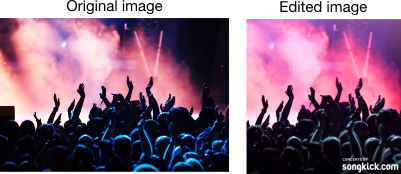
\includegraphics[height=60mm]{example2.png}
                  \caption{Before and after gimpifying.}
                \end{figure}


                When a user hovers their mouse over the two lower boxes, is animated to dim. This is achieved using an anchor html tag that is given the class boxClickUrl that expands the anchor to cover the entire parent. Also, the dim effect is achieved by setting the opacity of the image to a smaller value, revealing the black shadowbox behind.

            \subsubsection{Search Panel}
                From left to right in the search panel, we have a Google material icons search icon. Adjacent to the icon is an input box with placeholder text to indicate it is a search input. At the end, there are two date pickers produced using the \href{https://github.com/dbushell/Pikaday}{Pikaday} library. These allow the user to specify the query's date range.

                The previous items are positioned using the float CSS attribute so that each item is placed on the right of the previous one. Padding is set in various places to produce a pleasing result.  To create spaces between input boxes and text, non-breaking spaces are used. Date pickers, on hover, change the cursor to a pointer to indicate that they are clickable.

                For the search results, an empty list container is added for the search results to populate. A border-bottom is added to each list item as a border to separate results. Using the CSS selector last-child, we remove the last border-bottom so that the last list element does not have an end border.

                A custom calendar icon was created using two divs: the white-background class inside the red one. These are created using JavaScript, and it populates them with the required day and month.

                Initially, the Pikaday library did not work in strict xhtml mode due to a bug in the library that we have fixed and filed a \href{https://github.com/dbushell/Pikaday/pull/526}{pull request} for. We initialised two of these calendars by specifying the default date range. Also, when a user clicks a date from the from calendar, all dates before the current date are disabled to prevent them from selecting events from the past.

            \subsubsection{Map}
                Using the Google Maps API, we draw a map with a custom theme set to match the colour scheme of the  website. Also, we use Google map markers for our visualising event locations but we add our own custom SVG as their icons. To create these, a basic SVG marker was found off the Internet. Next, by using Inkscape's \"break apart\" tool, we deleted the opaque center to produce a transparent hole in the center of the marker. Lastly, the  marker is animated using Google's \"BOUNCE" animation setting.

                When animating these markers, we noticed that they would bounce in Safari and Firefox but not Chrome. Stepping through the markers script led to a getElementsByTagName looking for a HEAD tag in caps. Under XHTML, tags are case-sensitive and should always be lower case. However, in Firefox and Safari, the browser understood that this call was looking for the lower-case head tag. But this was not the case for Chrome as the query would produce no results. Attempting to change the sites head tag to upper-case did not solve the problem as different parts of Google's script made queries to find the head tag in lower case. The only valid solution found for this problem was to have two heads: one upper-case and one lower. This means we fail to meet the XHTML spec, but the marker animations work and the page is still rendered in the mentioned browsers. 

        \subsection{Logic}
            Main.js handles all of the logic for the web application. We subscribe to the window onload event as well as the Google Maps callback. In the window onload event, important functionality is setup such as the callbacks for the SVG button, intialise the websocket to the server, and initialising the date filter boxes.

            When the map has loading, the browser provides its location via the Google Maps API. This information is then used to setup the purple marker which indicates the user's position. After the map loads and websocket opens, the user's location is sent to the server via the websocket. This prompts the server to find nearby events and this information to be send back to the client.

            Afterwards, an array of events is received and thus we populate our internal events array. Next, using this information, we initialise the marker for each event. Also, a query is made to find the walking time to each of the events. Once the query has completed, the user can now click on the markers to display the info bar or search for events.

            To produce the sliding effect of the info panel, a class is swapped out of the sidebar when a user clicks a marker to give it a new margin-right property. As the info panel has a transition property, the slide in will be animated. The same thing is done with the Play button and Spotify player but with CSS properties background-color and padding-bottom to change the background colour of the play button and to show the Spotify player respectively.

            Whilst inputting the info panel with the relevant event information, a thumbnail for each artist needs to be created. To do this, we create a div with class bandimage for each artist and orderly append each one to the bandpics div which is the thumbnail container. This allows for a dynamic creation of thumbnails  as there can be any number of artists. Furthermore, the Spotify player's track URL is updated to load the correct song.

            To retrieve a string representing the search each time a new key is pressed, the keyup event is subscribed to the search bar. This event is then used to update the search results. First, the current query string is used to do a sublime-styled fuzzy search on each of the first and second artist names in every event. The fuzziness refers to the lack of matching sequential characters and thus there can be skips before matching. To visualise these matches, the result of the search wraps each matched character with a bold html tag. This means that when the search results are displayed, it can be clearly seen which characters in the artist names are produced the match.

            Event date, artist titles, and the walking time from the current location are included in the search data. For each result, a list element is created that contains a visualisation of the date, ordering of artist names, and walking time. Furthermore, these list items are appended to a html list element that exists in the existing html.

    \section{Server}
        On the server side, we used the provided script with modifications. The index is served as a static file and dynamic content is achieved using Websocket connections between the client and server. This design choice simplifies the file resource serving logic and thus reducing the dynamic parts to message passing.

        Once the client has initialised the webpage, it sets up a secure Websocket connection to the server. A secure socket is preferred as non-secure sockets are prevented when viewing the page over https. This connection is abstracted into websocket.js such that server.js can simply pass a callback.  This is called when a new client query is made. Also, passing a function which can be called with a result. 

        The browser's current geographical location is sent to the server along with the desired date range. Eventually, the server will reply with an array of events.

        Soon, the server will receive this data and use it to query the database using a geoNear query on a \href{https://docs.mongodb.com/manual/core/2dsphere/}{2dsphere} index. A similar query is performed on the date range on the event date. Afterwards, the results are sent back to the client.

        Since node does not come with a native websocket library, a popular third-party library was used: \href{https://github.com/theturtle32/WebSocket-Node}{theturtle32/WebSocket-Node}. Websockets provide a stream of messages, where a message is either some binary data or a string. We serialize JSON for sending data between the client and server. When the client sends its position and desired date range, we serialize a data structure that is defined by the following:

        \begin{verbatim}
        {
            pos: {
                lat: Number,
                lng: Number
            },
            dateRange: {
                from: Date,
                to: Date
            }
        }
        \end{verbatim}

        Dates are not parsed into JavaScript Date objects when using a JSON.parse so these are handled manually for the database queries.

        In addition to giving the client the desired data from the database, the database is checked to see whether it requires updating. This data is collected using a variety of APIs. First, the Songkick API is queried for the area that the user is in. This allows us to check the database to see if we have updated this area at all/recently. If the events for this area have not been updated recently, the events for the area are downloaded. In addition, last.fm is queried for artist biographies and pictures, Spotify for a reference to the artists' Spotify pages, and Google's reverse geocode API to get the full address of the venue.

        For each area we limit the frequency of requests in order to avoid rate limiting. Any errors returned by the APIs are handled graciously. Once complete, event data is retrieved, and stored in the database using an \href{https://docs.mongodb.com/manual/reference/method/db.collection.update/#upsert-option}{upsert} on the event title. This is done to either update an already queried event, or insert a new event.

        A possible optimization of the client-server interaction process would be to determine what events have already been sent to the client. This would avoid sending events again if the user scrolls the map slightly. As a result, this would allow for significantly less data to be transferred between the two and thus would avoid reprocessing every event on the client side.

        As we do not store any private data, encryption is not required for the data stored or obfuscated in any way. Validating the data retrieved from the client is necessary to stop a server crash. Additionally, location data is always sent over a secure websocket in order to prevent snooping.

    \section{Deployment}
        Since the server is written using some ES6 features, it requires a newer version of nodejs to run. By default, the server connects to a local mongojs server with no special configuration added. This implementation favours root accessible vps' such as digital ocean or \href{https://aws.amazon.com/ec2/}{EC2}.

        The development workflow consisted of a digital ocean instance that was setup with a bare git repo. Git hooks were written so that when a push to the repo is made, a clone of the repo is updated. Additionally, a call to npm install is made in order to update and install any libraries. On the server, the server script is run using \href{https://github.com/remy/nodemon}{nodemon} so that when the repo is updated, the server will restart.  

        This allows very fast staging tests, however this isn't suitable for a production run of the server. The site should be live at \href{https://smple.uk}{https://smple.uk}.

        Due to security issues, some browsers will not connect a secure websocket with an invalid certificate. Furthermore, the site is tested to be working on chrome locally for both https and http. When run with a valid certificate, everything works as it should.

    \section{API Usage}
        As we are using a few public APIs, we needed to take into consideration the terms for each of these:
        \begin{itemize}
            \item The Songkick API requires attribution when using their data in the form of a graphic they provide. We accommodated for this by adding their graphic into our ticket purchase button.

            \item The Spotify API has no requirement for the use of their embedded player as it already advertising where the player comes from.

            \item The last.fm API requires a link to their site on any information that is retrieved from them.  The retrieved biography includes a link to their website thus meeting the terms and conditions.
        \end{itemize}
\end{document}


